\documentclass[11pt,]{article}
\usepackage{lmodern}
\usepackage{amssymb,amsmath}
\usepackage{ifxetex,ifluatex}
\usepackage{fixltx2e} % provides \textsubscript
\ifnum 0\ifxetex 1\fi\ifluatex 1\fi=0 % if pdftex
  \usepackage[T1]{fontenc}
  \usepackage[utf8]{inputenc}
\else % if luatex or xelatex
  \ifxetex
    \usepackage{mathspec}
  \else
    \usepackage{fontspec}
  \fi
  \defaultfontfeatures{Ligatures=TeX,Scale=MatchLowercase}
\fi
% use upquote if available, for straight quotes in verbatim environments
\IfFileExists{upquote.sty}{\usepackage{upquote}}{}
% use microtype if available
\IfFileExists{microtype.sty}{%
\usepackage{microtype}
\UseMicrotypeSet[protrusion]{basicmath} % disable protrusion for tt fonts
}{}
\usepackage[margin=1in]{geometry}
\usepackage{hyperref}
\hypersetup{unicode=true,
            pdftitle={Supporting Information},
            pdfborder={0 0 0},
            breaklinks=true}
\urlstyle{same}  % don't use monospace font for urls
\usepackage{graphicx,grffile}
\makeatletter
\def\maxwidth{\ifdim\Gin@nat@width>\linewidth\linewidth\else\Gin@nat@width\fi}
\def\maxheight{\ifdim\Gin@nat@height>\textheight\textheight\else\Gin@nat@height\fi}
\makeatother
% Scale images if necessary, so that they will not overflow the page
% margins by default, and it is still possible to overwrite the defaults
% using explicit options in \includegraphics[width, height, ...]{}
\setkeys{Gin}{width=\maxwidth,height=\maxheight,keepaspectratio}
\IfFileExists{parskip.sty}{%
\usepackage{parskip}
}{% else
\setlength{\parindent}{0pt}
\setlength{\parskip}{6pt plus 2pt minus 1pt}
}
\setlength{\emergencystretch}{3em}  % prevent overfull lines
\providecommand{\tightlist}{%
  \setlength{\itemsep}{0pt}\setlength{\parskip}{0pt}}
\setcounter{secnumdepth}{0}

%%% Use protect on footnotes to avoid problems with footnotes in titles
\let\rmarkdownfootnote\footnote%
\def\footnote{\protect\rmarkdownfootnote}

%%% Change title format to be more compact
\usepackage{titling}

% Create subtitle command for use in maketitle
\newcommand{\subtitle}[1]{
  \posttitle{
    \begin{center}\large#1\end{center}
    }
}

\setlength{\droptitle}{-2em}
  \title{Supporting Information}
  \pretitle{\vspace{\droptitle}\centering\huge}
  \posttitle{\par}
  \author{}
  \preauthor{}\postauthor{}
  \date{}
  \predate{}\postdate{}

% load packages
\usepackage{amsmath,amsfonts,float,makecell,titletoc,titlesec,tocloft,lineno,booktabs,subfiles}
\usepackage[T1]{fontenc}
\usepackage{lmodern}
\usepackage[utf8]{inputenc}
\usepackage[doublespacing]{setspace}

% format captions
\usepackage[labelfont={small,bf}, labelsep=space, font={small}]{caption}

% line numbers
\linenumbers

% allow breaks in equations
\allowdisplaybreaks

% format abstract
\renewcommand{\abstractname}{Summary}
\renewenvironment{abstract}
 {\small
  \begin{center}
  \bfseries \abstractname\vspace{-.5em}\vspace{0pt}
  \end{center}
  \list{} {%
   \setlength{\leftmargin}{2mm}
   \setlength{\rightmargin}{\leftmargin}%
  }%
  \item\relax}
{\endlist}

% format section headers
\titleformat*{\section}{\Large\bfseries}
\titleformat{\subsection}[display]
	{\large\sffamily\lsstyle}
	{\subsectiontitlename\ \thesubsection}
	{0.5em}{}
\titleformat*{\subsubsection}{\large\itshape}

% make figures static
\let\origfigure\figure
\let\endorigfigure\endfigure
\renewenvironment{figure}[1][2] {
	\expandafter\origfigure\expandafter[H]
} {
	\endorigfigure
}

% define struts for tables
\newcommand\T{\rule{0pt}{2.6ex}} % top strut
\newcommand\B{\rule[-1.2ex]{0pt}{0pt}} % bottom strut

% define command to put new lines in table cells
%\newcommand{\specialcell}[2][c]{%
%  \begin{tabular}[#1]{@{}c@{}}#2\end{tabular}}

\begin{document}
\maketitle

\setcounter{figure}{0} \setcounter{table}{0}
\renewcommand{\thefigure}{S\arabic{figure}}
\renewcommand{\thetable}{S\arabic{table}}

\section{Appendix S1}\label{appendix-s1}

The reliable formulation explicitly considers the probability that
planning units are inhabited by features. As a consequence, it may
deliver prioritizations that will sufficiently represent an attribute
space even if the features do not inhabit several of the planning units
when the prioritization is implemented. This behavior is achieved by
siting back-up planning units near selected planning units with low
occupancy probabilities in the attribute space(s). To ensure that
prioritizations are robust against multiple planning units being
uninhabited, the problem assigns planning units at multiple backup
levels.

Backup levels levels are defined as \(r\)-levels (similar to failure
levels in Snyder \& Daskin 2005). The first backup \(r\)-level is used
to calculate the level of representation when all of the selected
planning units are occupied by all \(f \in F\). For this scenario, the
closest selected planning unit to each demand point \(i\) for attribute
space \(s\) is assigned at \(r\)-level\(=0\). This scenario essentially
represents \(Y_{fsij}\) in the unreliable formulation. The second backup
\(r\)-level is used to assess the level of representation when the
closest planning unit to each demand point \(i\) is unoccupied. For this
scenario, the second closest planning units are assigned at
\(r\)-level\(=1\). The third backup \(r\)-level is used to assess
representation when the first two closest planning units are unoccupied.
The third closest planning units are assigned at \(r\)-level\(=2\).
Continuing on, in this manner, the selected planning units in a
prioritization are assigned to each demand point \(i \in I\), attribute
space \(s \in S\), and each feature \(f \in F\) at an \(r\)-level.

A final backup \(r\)-level when \(r=R\) is used to assess the level of
representation when the features \(f \in F\) do not occupy any selected
planning units in a prioritisation. Each demand point \(i \in I\) for
each \(s \in S\) and \(f \in F\) is assigned to an ``imaginary''
planning unit \(j=J\) at \(r=R\). The distance variables associated with
this imaginary planning unit \(d_{fsiJ}\) denote the loss of biological
value associated with failing to secure a representative sample of
feature \(f\) in attribute space \(s\). However, the \(d\) variables are
in distance units which effectively meaningless in this context. Thus
these variables are calculated using a failure multiplier (\(M\)) and
the maximum distance between the planning units and the demand points
for \(f \in F\), \(s \in S\) (eqn 5).

\begin{align*}
& d_{fsiJ} = M \max\limits_{0 \leq i \leq I-1, 0 \leq j \leq J-1} d_{fsij} & \forall & 0 \leq f \leq F-1, \tag*{eqn 5} \\
& & & 0 \leq s \leq S-1\\
\end{align*}

Conservation planning problems often use more than several hundred
planning units. It is currently not be feasible to solve this problem
when considering all possible failure scenarios within a reasonable
amount of time (see Appendix S2). As a consequence, the \(R\) variable
can be any \(1 \leq R \leq J-1\). For instance, when \(R=3\) only 2
backup levels are considered in addition to the final backup level. Cui
\emph{et al.} (2010) found that \(R=5\) yields similar solutions to
\(R >> 5\). However, in most cases the decision maker will likely be
limited to \(R=1\) to obtain prioritizations in a feasible amount of
time.

The control variables for the reliable formulation are the \(B\) (eqn
1a), \(T_{s}\) (eqn 1b), \(\tau_{fs}\) (eqn 1c), \(R\), and \(M\)
variables.

\begin{align*}
R &= \parbox{25em}{number of failure levels} \tag*{eqn 6a} \\
%
M &= \parbox{25em}{failure multiplier} \tag*{eqn 6b}\\
%
\end{align*}

The decision variables are the \(X_j\) (eqn 2a), \(Y_{fsijr}\),
\(P_{fsijr}\) variables.

\begin{align*}
Y_{fsijr} &= \begin{cases}
    1, & \parbox{25em}{if demand point $i$ is assigned to planning unit $j$ for feature $f$ in space $s$ at back-up level $r$. } \tag*{eqn 7a} \\
    0, & \parbox{25em}{otherwise} \\
  \end{cases} \\
%
P_{fsijr} &= \parbox{25em}{probability that demand point $i$ is assigned to planning unit $j$ at back-up level $r$ for feature $f$ and space $s$} \tag*{eqn 7b}\\
%
\end{align*}

The reliable formulation (RRAP) is a multi-objective optimization
problem.

\begin{align*}
& \text{(RRAP)} & \text{Min } & \text{(3a)}\\
%
& & \text{s.t. } & \text{(3b)}\\
%
& & & 1 - \frac{\sum_{i=0}^{I-1} \sum_{j=0}^{J-1} \lambda_{fsi} {d_{fsij}}^{2} P_{fsijr} Y_{fsij}}{\sum_{i=0}^{I-1} \lambda_{fsi} {\delta_{fsi}}^{2}} \geq T_{fs}  & \forall & 0 \leq f \leq F-1, \tag*{eqn 8a}\\
& & & & & 0 \leq s \leq S-1\\
%
& & & \sum_{j=0}^{J-1} Y_{fsijr} = 1 & \forall & 0 \leq f \leq F-1, \tag*{eqn 8b}\\
& & & & & 0 \leq s \leq S-1,\\
& & & & & 0 \leq i \leq I-1,\\
& & & & & 0 \leq r \leq R\\
%
& & & \sum_{r=0}^{R} Y_{fsijr} = 1 & \forall & 0 \leq f \leq F-1, \tag*{eqn 8c}\\
& & & & & 0 \leq s \leq S-1,\\
& & & & & 0 \leq i \leq I-1,\\
& & & & & 0 \leq j \leq J\\
%
& & & \sum_{r=0}^{R-1} Y_{fsijr} \leq X_j & \forall & 0 \leq f \leq F-1, \tag*{eqn 8d}\\
& & & & & 0 \leq s \leq S-1,\\
& & & & & 0 \leq i \leq I-1,\\
& & & & & 0 \leq j \leq J-1\\
%
& & & Y_{fsiJR} = 1 & \forall & 0 \leq f \leq F-1, \tag*{eqn 8e}\\
& & & & & 0 \leq s \leq S-1,\\
& & & & & 0 \leq i \leq I-1\\
%
& & & P_{fsij0} = q_{fj} & \forall & 0 \leq f \leq F-1, \tag*{eqn 8f}\\
& & & & & 0 \leq s \leq S-1,\\
& & & & & 0 \leq i \leq I-1,\\
& & & & & 0 \leq j \leq J\\
%
& & & P_{fsijr} = \left(1 - \right) \sum_{k=0}^{J-1} \frac{1 - q_k}{q_k} P_{f,s,i,k,r-1} Y_{f,s,i,k,r-1}  & \forall & 0 \leq f \leq F-1, \tag*{eqn 8g}\\
& & & & & 0 \leq s \leq S-1,\\
& & & & & 0 \leq i \leq I-1,\\
& & & & & 0 \leq j \leq J,\\
& & & & & 1 \leq r \leq R\\
%
& & & X_j, Y_{fsijr} \in {0,1} & \forall & 0 \leq f \leq F-1, \tag*{eqn 8h}\\
& & & & & 0 \leq s \leq S-1,\\
& & & & & 0 \leq i \leq I-1,\\
& & & & & 0 \leq j \leq J,\\
& & & & & 0 \leq r \leq R\\
\end{align*}

The objective function for the reliable formulation is the same as for
the unreliable formation (eqn 3a). Similar to the unreliable
formulation, constraints (eqn 3b) and (eqn 8a) ensure that the
amount-based and space-based targets are met. Constraint (eqns 8b--7c)
ensure that each planning unit is only assigned to one backup
\(r\)-level for \(i \in I\). Constraints (eqn 8d) ensure that only
selected planning units are assigned to demand points \(i \in I\).
Constraints (eqn 8e) ensure that the imaginary planning unit is always
assigned to the highest backup \(r\)-level. Constraints (eqns 8f--8g)
determine the probability that planning unit \(j\) will be used to
sample demand point \(i \in I\) for \(s \in S\) and \(f \in F\) (see Cui
\emph{et al.} 2010 for more information). Constraints (eqn 8h) ensure
that the \(X\) and \(Y\) variables are binary.

The reliable formulation is non-linear. However, the non-linear
components can be linearized. First--as discussed in the main text--the
expression \(X_j X_k\) in (eqn 3a) can be linearized using methods
described by Beyer et al. (2016). Second, the expression
\(P_{fsijr} Y_{fsijr}\) in (eqn 8a) can be linearized using techniques
described by Sherali and Alameddine (1992) as implemented in Cui et al.
(2010).

\section{Appendix S2}\label{appendix-s2}

We conducted a benchmark analysis to understand how much time would be
required to build and solve different sized conservation planning
problems. Additionally, we also aimed to understand how the time
required to execute a problem varied depending on which formulation was
used (unreliable or reliable), and if fragmentation constraints were
used.

\subsection{METHODS}\label{methods}

We generated simulated conservation planning data sets using varying
number of features (c(10, 15, 20),c(10, 15, 20),c(10, 15, 20),c(10, 15,
20)) and planning units (c(10, 20, 30),c(10, 20, 30),c(10, 20, 30),c(10,
20, 30)). For a given number of planning units and features, the data
was simulated using the following steps. First, the planning units were
simulated as squares that were arranged in a grid. All planning unit
costs were set to one. The spatial distribution of features were
generated using binary, spatially autocorrelated random fields (using
the \texttt{RandomFields R} package; Schlather \emph{et al.} 2015,
2016). If features were associated with less than two occupied planning
units, these features were set to occupy two randomly selected planning
units. All occupied planning units were set to have a probability of
occupancy of 0.9. Similar to the simulated data sets used in the main
text, a geographic attribute space was used for each feature. The
features' demand points were set as the centroids of the planning units
that they occupied, and were weighted by the units' probability of
occupancy. All problems used amount-based targets of 20 \% and
space-based targets of 50

We solved each conservation planning data set using the unreliable and
reliable problem formulations (using default failure distance and level
parameter) using no boundary length modifier, and using a boundary
length modifier of 5. To assess variation in execution times, we
generated and solved 4 random data sets per combination of number of
features and planning units. All conservation planning problems were
solved to within 99 \% of optimality using Gurobi (version 7.0.0) on a
system with 64 GB RAM and an Intel(R) Xeon (R) CPU (E5-2630 v3; 2.40
GHz). All problems were solved using a single thread.

\subsection{RESULTS AND DISCUSSION}\label{results-and-discussion}

The benchmark analysis revealed that moderately-sized conservation
problems can be solved in a relatively short period of time (Figure S2).
As predicted, problems were solved much quicker when using the
unreliable formulation than when using the reliable formulation.
Additionally, the solve times varied substantially for different data
sets with the same properties (ie. number of features and planning
units). This result suggests that it may difficult to estimate exactly
how long a given problem will take to solve.

We were not able to explore how long large-sized problems would take to
solve because our computer system did not have enough memory. One method
to reduce the problem size would be to simply use less demand points.
Another method to reduce problem size would be to set a maximum distance
between demand points and planning units such that demand points cannot
be represented by planning units that that are too far away. Both of
these method could be applied using functions provided in the
\texttt{raptr R} package. Future research is needed to explore these
methods and understand how the impact solution quality. Additionally,
future research could involve implementing more advanced methods to
solve the optimization problems (eg. as described in Cui \emph{et al.}
2010; Aboolian \emph{et al.} 2013).

\clearpage

\section{Figures}\label{figures}

\begin{figure}
\centering
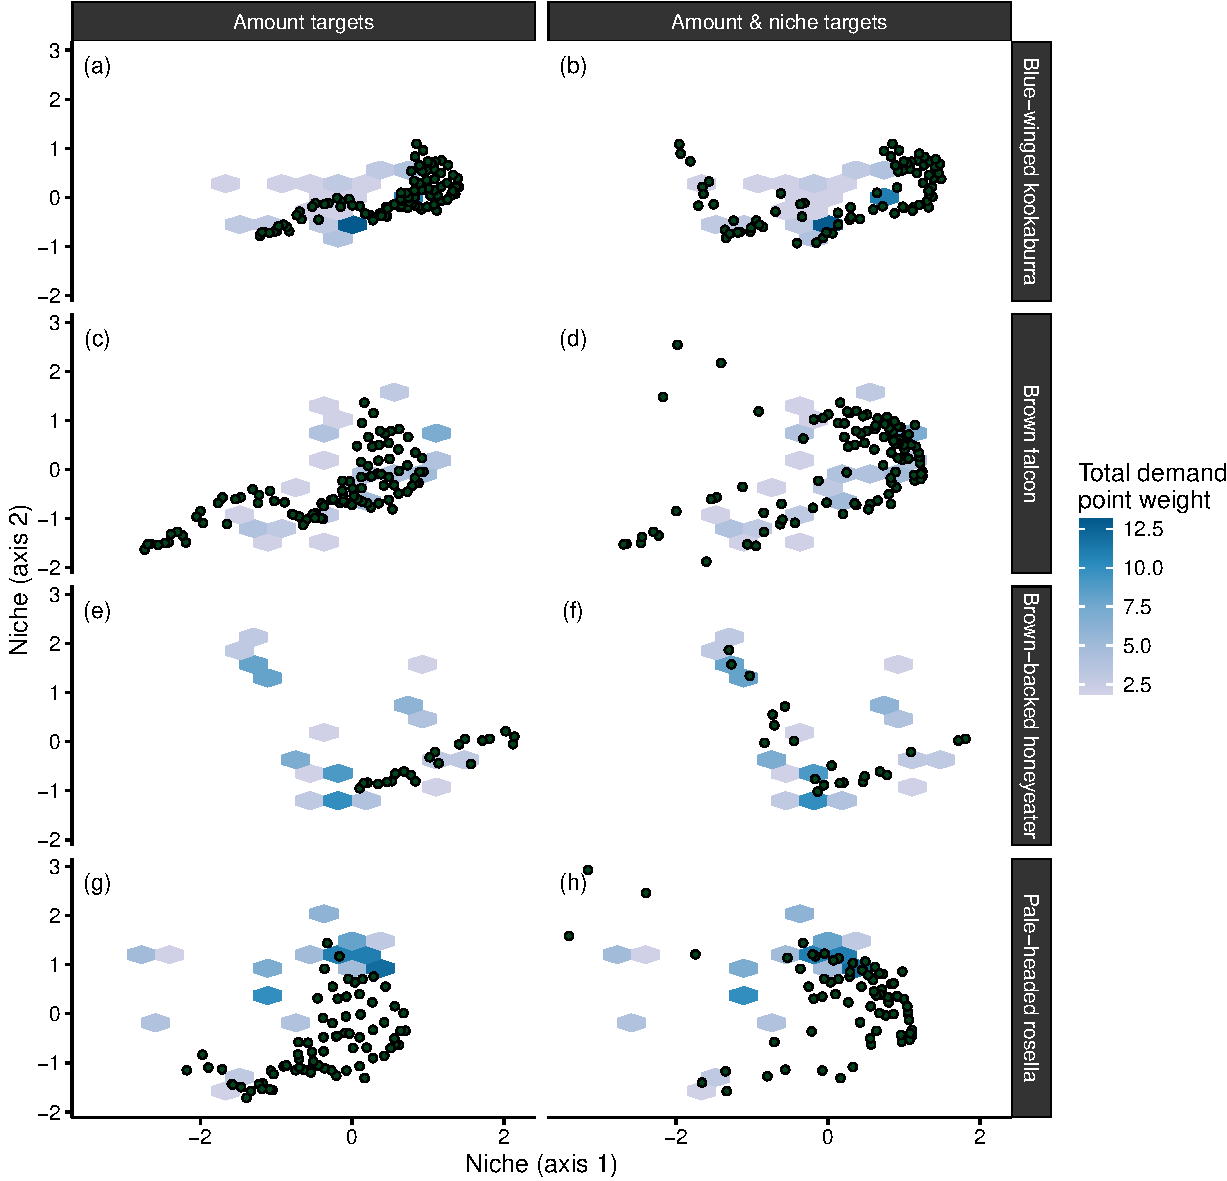
\includegraphics{supporting-information_files/figure-latex/unnamed-chunk-3-1.pdf}
\caption{Attribute spaces used in the first case-study. Each panel shows
a the distribution of a solution in environmental space and how it
samples the realized niche for a different species. The left column of
panels shows the solution generated using amount targets. The right
column of panels shows the solution generated using amount and niche
targets. Each column of panels corresponds to a different species.
Hexagons show the distribution of demand points. The color of each
hexagon denotes the weighted frequency of demand points inside it.
Points represent the environmental conditions associated with planning
units inside the species geographic range that were selected for
preservation in a given solution.}
\end{figure}

\begin{figure}
\centering
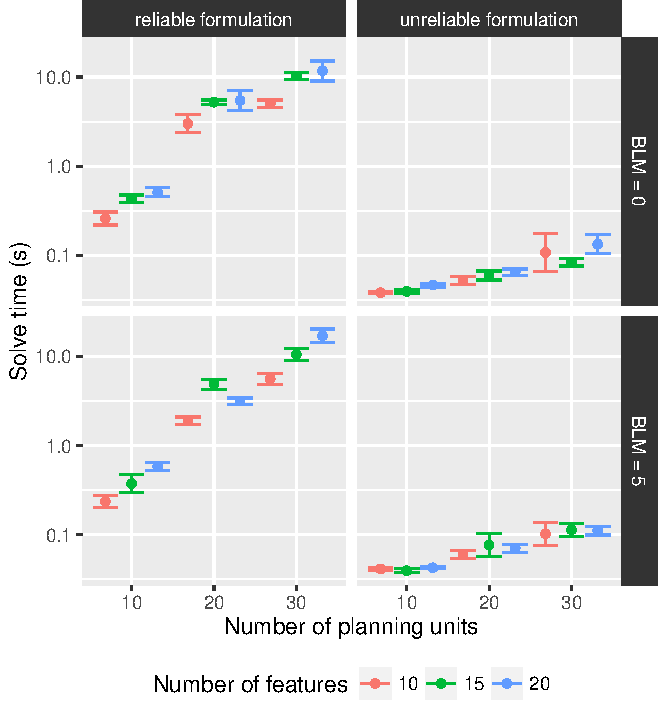
\includegraphics{supporting-information_files/figure-latex/unnamed-chunk-4-1.pdf}
\caption{Time required to solve different sized problems using different
parameters and formulations. Points represent average times and bars
show standard errors. Time is shown on a log\(_{10}\) scale.}
\end{figure}

\clearpage

\section{Tables}\label{tables}

\begin{table}[H]
\caption{Symbols and descriptions of terms used in the formulation of the unreliable representative and adequate prioritization (URAP) problem.\label{term}} 
\begin{center}
\begin{tabular}{cl}
\toprule[1pt]
\multicolumn{1}{c}{Symbol}&\multicolumn{1}{c}{Description}\tabularnewline
\midrule
$F$&\parbox[t][][t]{15cm}{set of biodiversity features (indexed by $f$)}\tabularnewline
$J$&\parbox[t][][t]{15cm}{set of planning units (indexed by $j$)}\tabularnewline
$q_{fj}$&\parbox[t][][t]{15cm}{probability of feature $f$ occupying planning unit $j$}\tabularnewline
$e_{jk}$&\parbox[t][][t]{15cm}{shared edge between planning unit $j$ and planning unit $k$. Note that when $j==k$ this used to parametrize exposed edges with no neighbours.}\tabularnewline
$S$&\parbox[t][][t]{15cm}{set of attribute spaces (indexed by $S$)}\tabularnewline
$I_{fsi}$&\parbox[t][][t]{15cm}{set of demand points (indexed by $i$) for a feature $f$ in attribute space $s$}\tabularnewline
$\lambda_{fsi}$&\parbox[t][][t]{15cm}{set of weights for demand point $i$ for feature $f$ in attribute space $s$}\tabularnewline
$d_{fsij}$&\parbox[t][][t]{15cm}{distance between demand point $i$ and planning unit $j$ for feature $f$ in attribute space $s$}\tabularnewline
$\delta_{fsi}$&\parbox[t][][t]{15cm}{the distance between each demand point $i$ and the centroid of the demand points $I$ for feature $f$ in attribute space $s$}\tabularnewline
$T_f$&\parbox[t][][t]{15cm}{amount target for feature $f$}\tabularnewline
$\tau_{fs}$&\parbox[t][][t]{15cm}{space-based target for feature $f$ in attribute space $s$}\tabularnewline
$X_j$&\parbox[t][][t]{15cm}{binary decision variable controlling if a planning unit is selected for preservation (1) or discarded (0)}\tabularnewline
$Y_{fsij}$&\parbox[t][][t]{15cm}{binary decision variable indicating if planning unit $j$ is assigned to demand point $i$ for species $s$ in a attribute space $s$ when determining the amount of the attribute space sampled by the selected planning units}\tabularnewline
\bottomrule[1pt]
\end{tabular}\end{center}
\end{table}

\clearpage

\subsection*{References}\label{references}
\addcontentsline{toc}{subsection}{References}

\hypertarget{refs}{}
\hypertarget{ref-r15}{}
Aboolian, R., Cui, T.T. \& Shen, Z.J.M. (2013). An efficient approach
for solving reliable facility location models. \emph{Informs Journal on
Computing}, \textbf{25}, 720--729.

\hypertarget{ref-r426}{}
Beyer, H.L., Dujardin, Y., Watts, M.E. \& Possingham, H.P. (2016).
Solving conservation planning problems with integer linear programming.
\emph{Ecological Modelling}, \textbf{328}, 14--22.

\hypertarget{ref-r16}{}
Cui, T.T., Ouyang, Y.F. \& Shen, Z.J.M. (2010). Reliable facility
location design under the risk of disruptions. \emph{Operations
Research}, \textbf{58}, 998--1011.

\hypertarget{ref-r494}{}
Schlather, M., Malinowski, A., Menck, P.J., Oesting, M. \& Strokorb, K.
(2015). Analysis, simulation and prediction of multivariate random
fields with package RandomFields. \emph{Journal of Statistical
Software}, \textbf{63}, 1--25.

\hypertarget{ref-r493}{}
Schlather, M., Malinowski, A., Oesting, M., Boecker, D., Strokorb, K.,
Engelke, S., Martini, J., Ballani, F., Moreva, O., Auel, J., Menck,
P.J., Gross, S., Ober, U., Christoph Berreth, Burmeister, K., Manitz,
J., Ribeiro, P., Singleton, R., Pfaff, B. \& R Core Team. (2016).
RandomFields: Simulation and analysis of random fields. R package
version 3.1.24.1, \url{https://cran.r-project.org/package=RandomFields}.

\hypertarget{ref-r20}{}
Sherali, H. \& Alameddine, A. (1992). A new reformulation-linearization
technique for bilinear programming problems. \emph{Journal of Global
Optimization}, \textbf{2}, 379--410.

\hypertarget{ref-r18}{}
Snyder, L.V. \& Daskin, M.S. (2005). Reliability models for facility
location: the expected failure cost case. \emph{Transportation Science},
\textbf{39}, 400--416.


\end{document}
